\documentclass{article}

\usepackage{authblk}
\usepackage{url}
\usepackage[square,numbers]{natbib}
\usepackage{amssymb,amsmath}
\usepackage[margin=1in]{geometry}
\usepackage{graphicx}
\usepackage{setspace}
\doublespacing

%\SectionNumbersOn
%\AbstractOn

\title{Exact Learning}
%\author{Benedict W. J.~Irwin}

\date{\today}
\begin{document}
%\bibliographystyle{harvard}

\author[1]{Benedict W. J.~Irwin}
\affil[1]{Machine Intelligence Group, Microsoft Research, Cambridge}
\affil[]{\textit {beirwin@microsoft.com}}


\maketitle

\begin{abstract}
Human mathematicians are very good at abstract reasoning. Computers are very good at large calculations. It has long been a goal to let computers deal in the abstract and symbolic patterns of mathematics.

Don't worry about too much peripheral stuff... i.e. neural networks etc. Easily do follow up papers...


We present a working machine learning method that can reverse engineer a wide class of numerical functions and write out exact mathematical expressions describing the underlying data.

This can be used for automated hypothesis generation, compiling tables of identities, assisting researchers as they work in an augmented fashion and ultimately one step closer to artificial intelligence working an reasoning with the space of analytic functions and performing exact, analytic mathematical tasks, attempting to understand complex data in high dimensions for example from particle physics/etc..

We give many examples.
We also attach a substantial theory document in the supplementary information.

Goal : 1D Examples
Goal : 2D Examples
Goal:   3,4,5,6,7D example.... Can we just fit a Lauricella function or similar...


Goal : Sparse data distributions?
Goal : Fitting with barely any samples/moments.
Goal : Connection of MGF to PDF/coefficients
Goal : CDF etc.

Goal : Tons of working examples.
Goal : Cumulant GF connection.

Eventual Goal: Modes of operation -> holonomic, products of functions ... etc.

\end{abstract}

%\tableofcontents

\section{Bigger Picture}
How do we find the mathematical rules behind our data? Many scientific fields have plots, curves and distributions that are not yet assigned an equation. We develop a framework to learn \underline{exact} mathematical solutions from numerical output. This could help researchers solve problems without having to solve equations.
In the long-term, developing such methods could lead to fundamental discoveries about our natural world. Can we learn complicated rules of physics and chemistry by spotting known functions in the data, and from this derive new theories?
We find an analogy between this method and the equations for neural networks that are already used today that gives a new perspective on the meaning of network parameters in existing models and could lead to advances in understandable AI. 





We present a collection of mathematical tools and emphasise a fundamental representation of analytic functions. Connecting these concepts leads to a framework for `exact learning', where an unknown numeric distribution could in principle be assigned an exact mathematical description. This is a new perspective on machine learning with potential applications in all domains of the mathematical sciences and the generalised representations presented here have not yet been widely considered in the context of machine learning and data analysis. The moments of a multivariate function or distribution are extracted using a Mellin transform and the generalised form of the coefficients is trained assuming a highly generalised Mellin-Barnes integral representation. The fit functions use many fewer parameters contemporary machine learning methods and any implementation that connects these concepts successfully will likely carry across to non-exact problems and provide approximate solutions. We compare the equations for the exact learning method with those for a neural network which leads to a new perspective on understanding what a neural network may be learning and how to interpret the parameters of those networks.


\section{Introduction}
This document summarises around eight years of work and represents a large development on top of an earlier preprint which laid down the foundations and mathematical concepts for exact learning. As this work was never published, we have attached it as the supplementary information of this document. However, for brevity we will only focus on new developments in the main text that allowed the idea to actually work in practice. 







First we reintroduce the motivation and goals of exact learning:


We will consider how in a broad sense `machine-learning-like-techniques' (i.e. advanced function fitting), can help with these `exact learning' type problems. Specifically for this work, the problem description is: 
\begin{enumerate}
\item[A)] \textbf{`Given a high precision numeric output of an unknown multivariate function or distribution write the `human readable equation' for that function as output, where it is possible to do so."}
\end{enumerate}
The concession we are willing to take on this quite general goal is:
\begin{enumerate}
\item[B)] \textbf{`Given a high precision numeric output of an unknown multivariate distribution write the \emph{unique fingerprint} of the distribution.'}
\end{enumerate}

The key change in goal B) is the introduction of a `\emph{fingerprint}' of an arbitrary function as a well behaved and meaningful intermediate that can identify a distribution \footnote{We have focused on distributions for the time being for simplicity, but extensions to this method will cover functions which are not bound at infinity}. The word fingerprint is local to this text and should not be considered a general term. The goals A) and B) can be seen as reverse engineering processes for \emph{functions}. It might be helpful to first consider the analogy of reverse engineering for a simpler object such as a \emph{number}, something that is performed by tools such as Simon Plouffe's `inverse symbolic calculator' \cite{Plouffe1986} and other `inverse equation solvers' \cite{Munafo}. In these tools a user can enter a high precision number - e.g. 14.687633495788080676 - and the algorithm would return a plausible closed form solution - e.g. $\pi^2 + e\sqrt{\pi}$. Once the user has the solution, the hope is that a human expert could use that extra information to come up with further insights which would assist in the scientific understanding of both the solution and problem.\\ 

Figure \ref{fig:Outline} depicts an overview of the `exact learning' procedure for a \emph{function}. Throughout this work we cover the necessary tools to understand the steps in the blue boxes on the right-hand side of this figure. Goal A) corresponds to the bottom left box, and goal B) is the bottom right box. The numeric data are collected from a natural source such as a very high-quality experiment, but more likely a numerical solution to a computational problem, or equation, or simulation. The solution is numerically transformed to `fingerprint space' (blue) by using an integral transform. The regularity of the representation of many analytic functions in this space assists with the fitting of the `fingerprint' using machine learning techniques to an assumed, highly generalised form. To get back to the mathematical expression of the solved function an inverse transformation is taken from the  fingerprint space to the function space. For examples of problems that might be interesting to solve using this method, please refer to the supplementary information. \\

\begin{figure}[h]
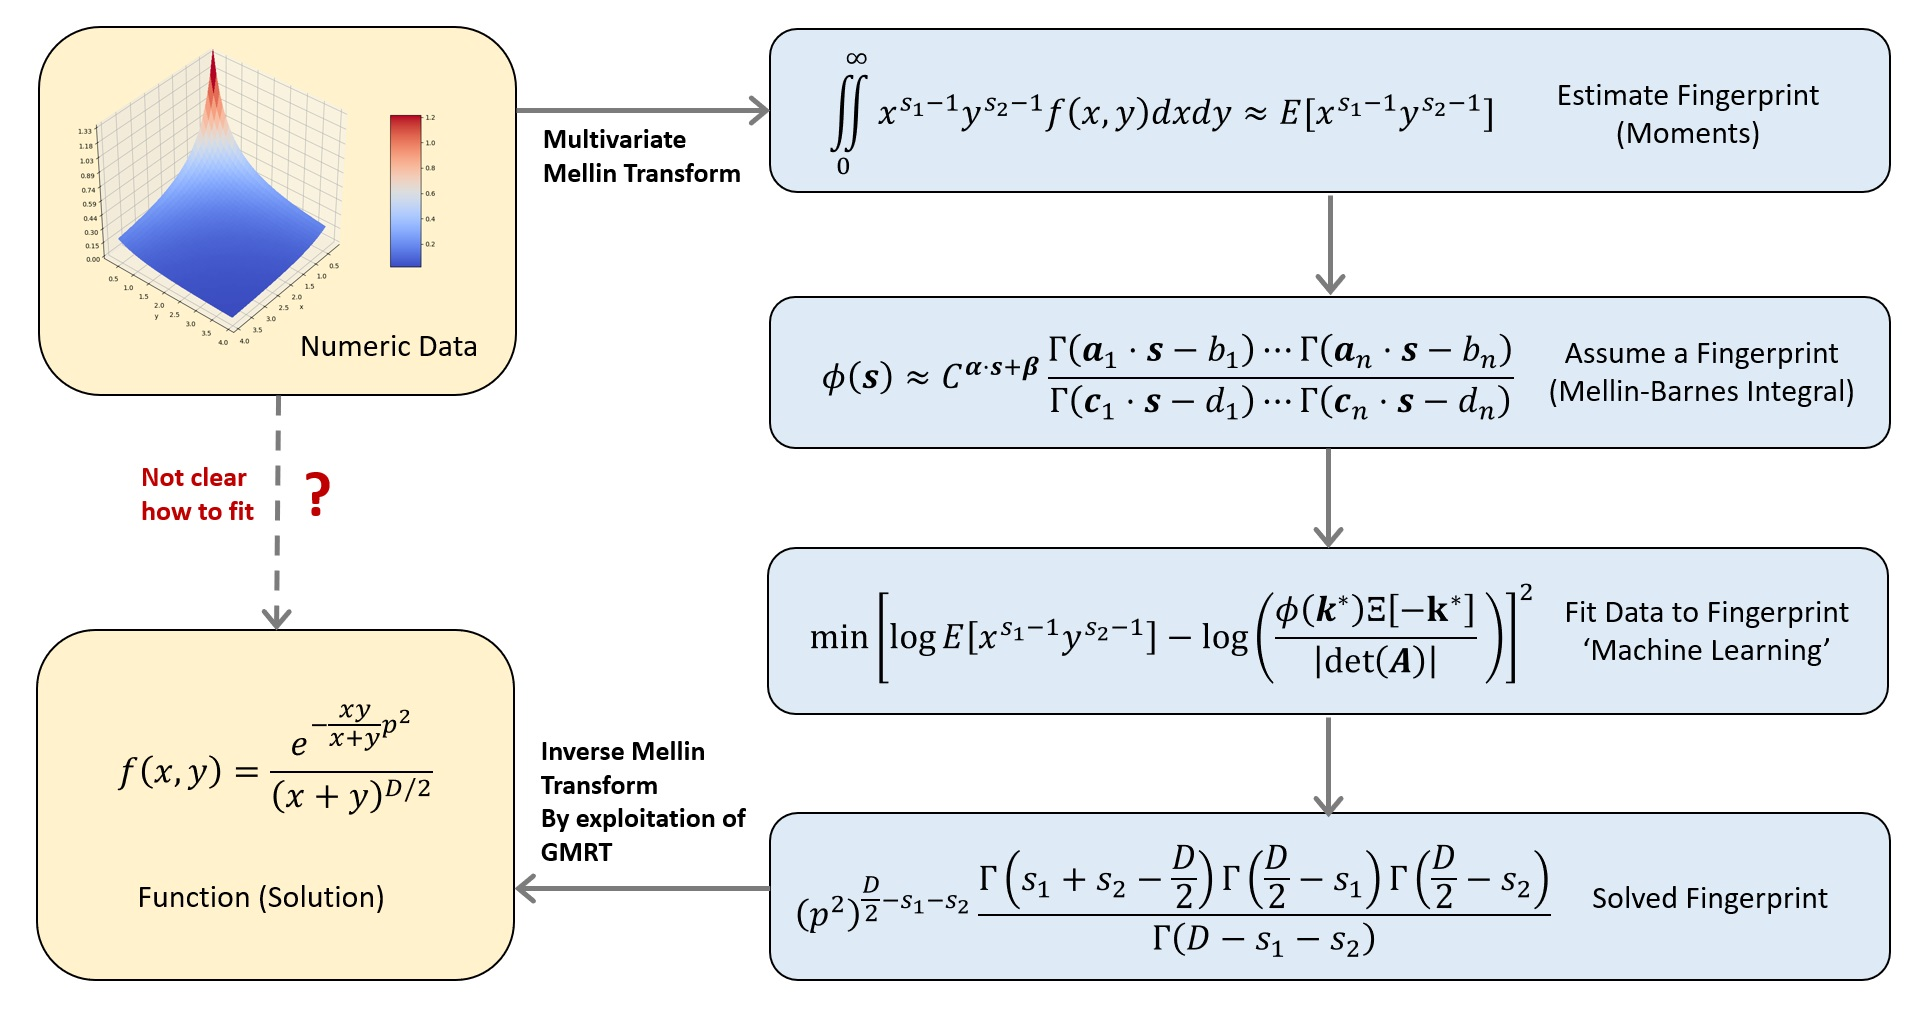
\includegraphics[scale = 0.323]{Figure1.jpg}
\caption{An example of the exact learning process, in this case with an example of the kernel of the massless Feynman bubble calculation given by Gonzalez et al. \cite{Gonzalez2015}. (Top left), A high precision numerical function is found as the solution to a problem that likely has an analytic solution, but the closed form is hard to derive mathematically. A numeric Mellin transform is made from the `function domain' (yellow) into the `fingerprint domain' (blue) for a number of chosen exponent vectors $\mathbf{s}=(s_1,\cdots,s_2)$. A highly generalised closed form for the fingerprint is chosen and then machine learning (function fitting) is used to track down the parameters of the function fingerprint ($\mathbf{a,b,c,d}$). With further analysis and interpretation of the solved parameters the fingerprint could be used to derive the closed form for the function that generated the original numeric data using the generalised Ramanujan master theorem (GMRT).}
\label{fig:Outline}
\end{figure}

\section{Theoretical Justification}
Unique moments : Discussion of three kind of moment problem $[0,\infty)$, $(-\infty,\infty)$ and $[a,b]$ with $[0,1]$ as a special case. Reference higher dimensional moment problem example. Try to link existence of CF via MGF via Mellin transform definition. Answer, if the moments converge, then the Mellin transform would converge, then the thing would exist, so they are unique... up to strip of holonomy?

Connection between coefficients, PDF, series coefficients MGF, CF, Mellin transform, cumulant GF.

Log-convex for many functions.

Solutions of differential equations. holonomic functions, annihilation operator, Mellin transform. etc.

\section{Multidimensional Examples}
For general analytic multivariate functions, the moments/series coefficients can be exposed through the Ramanujan Master Theorem as
$$
RMT
$$
Where the multivariate function can be expressed as a product of univariate functions with known Mellin transforms and with argument as a multivariate monomial term, it is possible to construct a general rule of thumb where the order of integration in the Mellin transform does not matter. As this was derived experimentally by the author, we call this Irwin's Master Theorem for lack of a better name.
$$
\mathcal{M}_D\left[\prod_{k=1}^n f_k \left(\alpha_k \prod_{l=1}^n x_l^{a_{kl}}\right) \right]=\frac{\prod_{k=1}^n \alpha_k^{-(A^\top)_k^{-1} \mathbf{s}}}{|\det(\mathbf{A})|} \prod_{k=1}^n g_k((A^\top)_k^{-1} \mathbf{s})
$$

Here $\mathbf{A}$ is a matrix with elements $a_{kl}$. If $\mathbf{A}$ is singular, the expression does not exist. A non-square, singular value equivalent expression may exist. [See Appendix Section XYZ for an example.]. This rule of thumb, allows us to check the algorithm is working.

For an increasingly generalised example of this we have 
$$
\mathcal{M}_D\left[  \mathbf{x}^{\mathbf{b}}\partial_{\mathbf{x}}^{\mathbf{q}} \prod_{k=1}^n f_k \left(\alpha_k \prod_{l=1}^n x_l^{a_{kl}}\right) \right](\mathbf{s})= \frac{\prod_{k=1}^n \alpha_k^{-(A^\top)_k^{-1} (\mathbf{s-q})}}{|\det(\mathbf{A})|} \left[\prod_{k=1}^n  g_k((\mathbf{A}^\top)_k^{-1} (\mathbf{s-q}))\right]\left[\prod_{k=1}^n \frac{(-1)^{s_k}\Gamma(s_k)}{\Gamma(s_k-q_k)}\right]
$$




\section{Note}
Consider taking derivatives of each function...
Derivatives can be taken with respect to each variable $x_1, \cdots, x_n$, on each function $f_k$, so we end up with something like

$$
\mathcal{M}_D\left[\prod_{k=1}^n f^{(\mathbf{q})}_k \left(\alpha_k \prod_{l=1}^n x_l^{a_{kl}}\right) \right]= \cdots
$$
where $\mathbf{q} = (0,1,0,2,1)$ would mean $\partial_2 \partial_4^2 \partial_5$

The normal Mellin transform rule is 
$$
\mathcal{M}[f'(x)](s) = (1-s)\phi(s-1)
$$
and
$$
\mathcal{M}[f^{(k)}(x)](s) = \frac{(-1)^k \Gamma(s)}{\Gamma(s-k)}\phi(s-k)
$$
and we do find an analogy to this, but now there is a vector $\mathbf{q}$, such that
$$
\mathcal{M}_D\left[\prod_{k=1}^n f^{(\mathbf{q}_k)}_k \left(\alpha_k \prod_{l=1}^n x_l^{a_{kl}}\right) \right](\mathbf{s})= \frac{\prod_{k=1}^n \alpha_k^{-(A^\top)_k^{-1} \mathbf{s}}}{|\det(\mathbf{A})|} \prod_{k=1}^n  g_k((\mathbf{A}^\top)_k^{-1} (\mathbf{s-q}_k))
$$
where we need to insert meaning to the vectorised version of a polynomial...[IT IS A PRODUCT for EACH elemtn of the vector, i.e. polynomial of different orders] and check that $\Sigma q$ is indeed the sum of the elements of the derivative vector.

All of the $\mathbf{q}_k$ together make a matrix $\mathbf{Q}$ which is the derivative order of each variable for each function.

If we have the original (undifferentiated version)
$$
\phi(\mathbf{s})
$$
then when we differentiate with a matrix $\mathbf{Q}$, where rows are the derivative order for each variable in one function. If we take the column sums we get a vector $\chi$. Then the new result is similar to $\phi(\mathbf{s-\chi})$, and the remaining terms are a series of factors that seem to depend on the rows $(A^\top)_k^{-1}$ and the Pochhamer type terms 
$$
\frac{(-1)^{q_k}\Gamma(\mathbf{s})}{\Gamma(\mathbf{s-q}_k)}
$$


Example
$$
f(x_1,x_2) = e^{-x_1+x_2}e^{-x_1 - x_2^2}
$$

Actually, we might be going too far with a matrix $Q$ and instead we could consider a bunch of partial derivatives applied to the whole function by the chain rule 
$$
\partial_{x_1}^{q_1} \cdots \partial_{x_n}^{q_n}
$$
this should look along the lines of
$$
\mathcal{M}_D\left[\partial_{x_1}^{q_1} \cdots \partial_{x_n}^{q_n}\prod_{k=1}^n f_k \left(\alpha_k \prod_{l=1}^n x_l^{a_{kl}}\right) \right](\mathbf{s})= \frac{\prod_{k=1}^n \alpha_k^{-(A^\top)_k^{-1} (\mathbf{s-q})}}{|\det(\mathbf{A})|} \left[\prod_{k=1}^n  g_k((\mathbf{A}^\top)_k^{-1} (\mathbf{s-q}))\right]\left[\prod_{k=1}^n \frac{(-1)^{s_k}\Gamma(s_k)}{\Gamma(s_k-q_k)}\right]
$$
and may ultimately be more useful because the function will only be evaluated numerically in some scenarios. We might then consider that because the Pochhammer type structure is predictable and general but the $\alpha_k$ type coefficients are not, if we could extract a form for the matrix $A$ by simply pinging off derivatives, without knowing the functions $g_k$, then once we had the matrix, we could removed the determinant factor, and try to reverse engineer the functions as a power series in the original domain, or as the coefficients for exact learning in the Mellin domain.

Beyond this, we can include additional polynomial type terms as
$$
\mathcal{M}_D\left[  \mathbf{x}^{\mathbf{b}}\partial_{\mathbf{x}}^{\mathbf{q}} \prod_{k=1}^n f_k \left(\alpha_k \prod_{l=1}^n x_l^{a_{kl}}\right) \right](\mathbf{s})= \frac{\prod_{k=1}^n \alpha_k^{-(A^\top)_k^{-1} (\mathbf{s-q})}}{|\det(\mathbf{A})|} \left[\prod_{k=1}^n  g_k((\mathbf{A}^\top)_k^{-1} (\mathbf{s-q}))\right]\left[\prod_{k=1}^n \frac{(-1)^{s_k}\Gamma(s_k)}{\Gamma(s_k-q_k)}\right]
$$




However, for matrix $Q$, there may be a useful interpretation in finding some complicated identity for an expression in terms of the derivatives of building blocks.


We could imagine a scenario where we have a multivariate and holonomic relationship on such a function, to create an annihilation operator.



\subsection{Super General}
Consider analogy
$$
\int \phi^{-1}\left(\phi\left(f_1\left(\phi^{-1}\left( a_{11}\phi(x_1) + a_{12}\phi(x_2) + a_{13} \phi(x_3) \right)\right) \right) + \phi() + \phi() \right)
$$
for generalisation of Mellin transform for $\phi$. Link this up to the Fourier transform for example, or an additive type/ general case when $\phi = 1$...

$$
\int \int \int f_1(a_{11} x_1 + a_{12} x_2 + a_{13} x_3) + f_2(a_{21} x_1 + a_{22} x_2 + a_{23} x_3) + f_3( a_{31} x_1 + a_{32} x_2 + a_{33} x_3) \; dx_1 d x_2 d x_3
$$
invoke Jacobian change of variables, $u_1 = \alpha x_1 + \beta x_2 + \gamma x_3$ ... 

Try to find this out for the general case of any functions!

N-D FourierTransform of a product of Gaussians, with argument linear in $x_1,x_2,x_3$, all coefficients in a big matrix, ends up being a large expression with terms equal to matrix (det, trace, elements ,minors) etc.



$$
A_2 = \begin{bmatrix}
a&b \\ c& d
\end{bmatrix}
$$

$$
A_3 = \begin{bmatrix}
a & b & c \\
d & e & f \\
g & h & i
\end{bmatrix}
$$
$$
F_2 = 
\frac{\exp \left(-\frac{(a_2 \cdot a_2 )t_1^2 + (a_1 \cdot a_1 ) t_2^2 -2 (a_1 \cdot a_2) t_1 t_2}{4 (\det A)^2}\right)}{2 \sqrt{a_1 \cdot a_1}
    \sqrt{\frac{(\det A)^2}{a_1 \cdot a_1 }}}
$$
    
$$
F_3 = \frac{AA}{BB}
$$

$$
AA = \exp(-pp/dd)
$$
$$
dd = 4 (\det A)^2
$$

\begin{align}
pp = \\
\text{t3}^2 \left(a^2 \left(e^2+h^2\right)+(e g-d h)^2\right)
-2 \text{t3} \left(a^2 \text{t2} (e f+h i)+\text{t1} (e g-d h) (e i-f h)+\text{t2} (e g-d h) (f g-d i)\right)\\
+a^2 f^2 \text{t2}^2 \\
+a^2 i^2 \text{t2}^2 \\
+2 c \text{t3} \left(a \text{t2} (d e+g h) -a \text{t1} \left(e^2+h^2\right)-b \text{t2} \left(d^2+g^2\right)+b \text{t1} (d e+g h)\right)
\end{align}

\begin{align}
-2 c (b\text{t1}-a \text{t2}) (-\text{t2} (d f+g i)+e f \text{t1}+h i \text{t1})
+2 a b \left(\text{t3} (d f \text{t2}+e f \text{t1}+g i \text{t2}+h i \text{t1})
-\left(\text{t3}^2 (d e+g h)\right)
-\text{t1}
    \text{t2} \left(f^2+i^2\right)\right) 
    +b^2 \left(\text{t3}^2 \left(d^2+g^2\right)-2 \text{t1} \text{t3} (d f+g i)+\text{t1}^2 \left(f^2+i^2\right)\right)+c^2 \left(\text{t2}^2 \left(d^2+g^2\right)
    -2\text{t1} \text{t2} (d e+g h)+\text{t1}^2 \left(e^2+h^2\right)\right)\\
\end{align}
 \begin{align}
    +d^2 i^2 \text{t2}^2\\
    -2 d e i^2 \text{t1} \text{t2}\\
    -2 d f g i \text{t2}^2\\
    +2 d f h i \text{t1} \text{t2}\\
    +e^2 i^2 \text{t1}^2\\
    + 2 e f g i \text{t1} \text{t2} \\
    -2 e f h i \text{t1}^2 \\
    +f^2 g^2 \text{t2}^2 \\
    -2 f^2 g h \text{t1} \text{t2} \\
    +f^2 h^2 \text{t1}^2
\end{align}    

$$    
BB = 2 \sqrt{2} \sqrt{a_1 \cdot a_1}
    \sqrt{\frac{tt}{a_1 \cdot a_1}} \sqrt{\frac{(\det A)^2}{tt}}
$$
$$
tt = a^2 \left(e^2+h^2\right)-2 a b (d e+g h)+b^2 \left(d^2+g^2\right)+(e g-d h)^2
$$

The polynomial has coefficients 
$$
[t_1^2] = b^2 \left(f^2+i^2\right)-2 b c (e f+h i)+c^2 \left(e^2+h^2\right)+(f h-e i)^2
$$
$$
[t_2^2] = a^2 \left(f^2+i^2\right)-2 a c (d f+g i)+c^2 \left(d^2+g^2\right)+(f g-d i)^2
$$
$$
[t_3^2] = a^2 \left(e^2+h^2\right)-2 a b (d e+g h)+b^2 \left(d^2+g^2\right)+(e g-d h)^2
$$
and 
$$
[t_1 t_2] =-2 \left(-c (a e f+a h i+b d f+b g i)+a b \left(f^2+i^2\right)+c^2 (d e+g h)+(f g-d i) (f h-e i)\right)
$$
$$
[t_2 t_3] = -2 \left(a^2 (e f+h i)-a b (d f+g i)-a c (d e+g h)+b c \left(d^2+g^2\right)+(e g-d h) (f g-d i)\right)
$$
$$
[t_3 t_1] = 2 b (a e f+a h i+c d e+c g h)-2 \left(a c \left(e^2+h^2\right)+(e g-d h) (e i-f h)\right)-2 b^2 (d f+g i)
$$


We apparently have the coefficient for $t_1^2$ is the sum of the first row of $(A^{-1})^2$, and

I.e. we have a term
$$
\begin{bmatrix}
t_1^2 & t_2^2 & t_3^2
\end{bmatrix}
\cdot A^{-2}
\cdot
\begin{bmatrix}
1 \\ 1 \\ 1
\end{bmatrix}
$$

This was Hadamard product/.


Define
$$
K = |\det A| A^{-1}
$$
let $k_i$ be the $ith$ row of $K$.
Then we end up with coefficients for $t_i t_j$ as 
$$
[t_i t_j] = k_i \cdot k_j + k_j \cdot k_i
$$
and
$$
[t_i t_i] = k_i \cdot k_i
$$


It is equal to 
$$
\mathbf{t} \cdot \mathbf{A A}^\top \cdot \mathbf{t}
$$
or if we keep the matrix as $(A^\top)^{-1}$ then it is
$$
\mathbf{t} \cdot \mathbf{A^\top A} \cdot \mathbf{t}
$$

So the product of $n$ Gaussian Fourier transforms looks like 
$$
\mathcal{F}_{n}\left[ \prod_{k=1}^n e^{-(\mathbf{a}_k\cdot\mathbf{x})^2} \right] = \frac{\exp\left(- \frac{\mathbf{t} \cdot \mathbf{((A^\top)^{-1})^\top (A^\top)^{-1}} \cdot \mathbf{t}}{4} \right)}{2^{n/2}|\det \mathbf{A}|}
$$

What this means, is the product on the left ends up being a fully correlated "Multivariate" Gaussian. And the fourier transform is of course, still a multivariate Gaussian, so we just have a new form for the covariance matrix, i.e. a decomposition.

This is great, because it helps us understand the multivariate pdf in terms of the Ramanujan master theorem etc...

\subsection{Next}
Next we can explore the generality of it, when dealing with a product of arbitrary mixture of functions... In a similar vein to the Mellin transforms.

Mixing $e^{-x}$ and $e^{-x^2}$ we get as expected a mixture

$$
\frac{\sqrt{\pi } e^{\frac{c^2}{4 a^2}-\frac{i c \text{t1}}{2 a^2}-\frac{\text{t1}^2}{4 a^2}} \delta \left(-\frac{i b c}{a}+i d-\frac{b \text{t1}}{a}+\text{t2}\right)}{\sqrt{a^2}}
$$

Inspecting the $(A^\top)^{-1}$

$$
(A^\top)^{-1} = \left(
                   \begin{array}{cc}
                    \frac{d}{a d-b c} & -\frac{c}{a d-b c} \\
                    -\frac{b}{a d-b c} & \frac{a}{a d-b c} \\
                   \end{array}
                   \right)
$$
 $$
            ((A^\top)^{-1})^\top (A^\top)^{-1} =      \left(
                   \begin{array}{cc}
                    \frac{b^2}{(a d-b c)^2}+\frac{d^2}{(a d-b c)^2} & -\frac{a b}{(a d-b c)^2}-\frac{c d}{(a d-b c)^2} \\
                    -\frac{a b}{(a d-b c)^2}-\frac{c d}{(a d-b c)^2} & \frac{a^2}{(a d-b c)^2}+\frac{c^2}{(a d-b c)^2} \\
                   \end{array}
                   \right)
                   $$
                   
Weirdly in this case the determinant appears to be been reduced to a single factor of $a$. We have the argument of the delta function having the bottom row of the matrix times $\mathbf{t}$, which is good to see.     

The argument of the exponential appears to be 
$$
(-i t_1 + \frac{c}{2 a})(-i t_1 + \frac{c}{2 a})
$$         

If we swap the mixture we get 
$$
\frac{\sqrt{\pi } e^{\frac{a^2}{4 c^2}-\frac{i a \text{t1}}{2 c^2}-\frac{\text{t1}^2}{4 c^2}} \delta \left(i b-\frac{i a d}{c}-\frac{d \text{t1}}{c}+\text{t2}\right)}{\sqrt{c^2}}
$$

When they are both simple exponentials we have 
$$
2 \pi  \delta (i a+i c+\text{t1}) \delta (i b+i d+\text{t2})
$$
so we apparently have some blending in going on. We might try another function.

\subsubsection{Example}



Because $\mathcal{M}[f(x)](s) = \mathcal{B}[f(e^{-x})](s)$ we can simply convert to bilateral Laplace transform
$$
\mathcal{M}_D\left[\prod_{k=1}^n f_k \left(\alpha_k \prod_{l=1}^n x_l^{a_{kl}}\right) \right](\mathbf{s})=\frac{\prod_{k=1}^n \alpha_k^{-(A^\top)_k^{-1} \mathbf{s}}}{|\det(\mathbf{A})|} \prod_{k=1}^n g_k((A^\top)_k^{-1} \mathbf{s})
$$
$$
\mathcal{B}_D\left[\prod_{k=1}^n f_k \left(\alpha_k \prod_{l=1}^n e^{-a_{kl}x_l}\right) \right](\mathbf{s})=\frac{\prod_{k=1}^n \alpha_k^{-(A^\top)_k^{-1} \mathbf{s}}}{|\det(\mathbf{A})|} \prod_{k=1}^n g_k((A^\top)_k^{-1} \mathbf{s})
$$

Consider a transform
$$
H_n = \int_0^1 \frac{1-x^n}{1-x} \; dx = \mathcal{T}\left[\frac{1}{1-x}\right]
$$

We have 
$$
\mathcal{T}[1] = \frac{n}{1+n}
$$

We might speculate that 
$$
\int_0^1\int_0^1\frac{(1-x^n)(1-y^n)}{(1- a x + b y)(1 - c x + d y)} \; dx dy \to H_{n_1} H_{n_2}
$$
type expression

Consider
$$
\int_0^1\int_0^1\frac{(1-x^{a n_1 + b n_2})(1-y^{c n_1 + d n 2})}{(1 - x)(1 - y)} \; dx dy = H_{a n_1 + b n_2}H_{c n_1 + d n 2}
$$
let
$$
u^{k_1} = x^{a n_1 + b n_2}
$$
$$
dx = \frac{k_1}{a n_1 + b n_2}u^{\frac{k_1}{a n_1 + b n_2} -1} du
$$

$$
H_{a n_1 + b n_2}H_{c n_1 + d n 2} = \frac{k_1 k_1}{(a n_1 + b n_2)(c n_1 + d n_2)} \int_0^1\int_0^1\frac{(1-u^{k_1})(1-v^{k_2})}{(1 - u^{\frac{k_1}{a n_1 + b n_2}})(1 - v^{\frac{k_2}{c n_1 + d n_2}})} \; u^{\frac{k_1}{a n_1 + b n_2} -1}  v^{\frac{k_2}{c n_1 + d n_2} -1} du dv
$$

Rather we might consider
$$
H_{\frac{a n_2 - b n_1}{\det A}}H_{\frac{d n_1 - c n 2}{\det A}} = \int_0^1\int_0^1\frac{(1-x^{\frac{a n_2 - b n_1}{\det A}})(1-y^{\frac{d n_1 - c n 2}{\det A}})}{(1 - x)(1 - y)} \; dx dy
$$

Note that 
$$
\int_0^1 \frac{1}{b}\frac{(1 - x^{a/b - 1})}{(1 - x^{1/b})} = \psi_0(a) - \psi_0(b)
$$


It seems the inverse transform is 'just' 
$$
-\sum_{res} x^{-s-1} \mathcal{T}[f(x)](s)
$$
such that 
$$
-\sum_{res} x^{-s-1} H_s = \frac{1}{1-x}
$$

It might be better to use
$$
-\sum_{res} x^{-s} \psi_0(s) = \frac{1}{1-x}
$$

This clearly relates to a harmonic equivalent of the hypergeometric series etc...


\section{Idea of Continous Power Series...}
Imagine 
$$
\frac{1}{n} \sum_{k=0}^n x^{k/n}
$$
as $n \to \infty$ we get 
$$
\int_0^1 x^k \; dk = \frac{x-1}{\log(x)}
$$
also
$$
\int_0^\infty x^k \; dk = \frac{-1}{\log(x)}
$$


There is no form for $n \to \infty$
$$
\frac{e^{x^{\frac{1}{n}}} \left((n+1) \Gamma \left(n+1,x^{\frac{1}{n}}\right)-((n+1) \Gamma (n+1))+\Gamma (n+2)\right)}{n \Gamma (n+2)}
$$
which is from the exponential equivalent
$$
\int_0^1 \frac{x^k}{\Gamma(k+1)} \; dk
$$

How do we get the coefficient 'function' out of the integral? For this 'continuous' Z-transform type thing... What is the continuous inverse transform? I.e. a type of residue to extract a function? 

Normally coefficients are linked to derivatives... Do the fractional derivatives help? 

We get the fractional derivative of 
$$
D_\alpha \frac{x-1}{\log(x)} = \frac{0^{-a-1} (\text{Ei}(2 \log (x))-\text{li}(x))}{\Gamma (-a)}
$$
which is clearly related to 
$$
\int_0^1 \frac{x^k}{k+1} \; dk = \frac{\text{Ei}(2 \log (x))-\text{li}(x)}{x}
$$

We can basically invent a functional inverse-Z transform such that 
$$
\mathcal{Z}^{-1}_F \left[\frac{(\frac{1}{x}-1)}{\log(\frac{1}{x})}\right] = 1
$$
and the forward is basically 
$$
\mathcal{Z}_F[g(k)] = \int_0^1 g(k) x^k \; dk
$$

now we have 
$$
\int_0^1 k^n x^k \; dx = \fbox{$(-\log (x))^{-n-1} (\Gamma (n+1)-\Gamma (n+1,-\log (x)))\text{ if }\Re(\log (x))<0\land \Re(n)>-1$}
$$
and 
$$
\int_0^\infty k^n x^k \; dk =  \fbox{$\Gamma (n+1) (-\log (x))^{-n-1}\text{ if }\Re(\log (x))<0\land \Re(n)>-1$}
$$
which has a special feeling (in terms of Mellin transform) for
$$
\mathcal{Z}_F[k^{n-1}] = \int_0^\infty k^{n-1} x^k \; dk = \fbox{$\Gamma (n) (-\log (x))^{-n}\text{ if }\Re(\log (x))<0\land \Re(n)>0$}
$$
and also
$$
\mathcal{Z}_F[k^{-n-1}] = \int_0^\infty k^{n-1} x^k \; dk = \fbox{$\Gamma (-n) (-\log (x))^n\text{ if }\Re(n)<0\land \Re(\log (x))<0$}
$$

We have 
$$
\int_0^\infty \sin(2 \pi k) x^k \; dk = \fbox{$\frac{2 \pi }{\log ^2(x)+4 \pi ^2}\text{ if }\Re(\log (x))<0$}
$$

So we would have that 
$$
\mathcal{Z}^{-1}_F \left[ \frac{2 \pi}{\log^2(\frac{1}{x}) + 4 \pi^2}\right] = \sin(2 \pi k)
$$
integrating this does seem to give sinintegral type results... So we may be close.. as 
$$
z D_z Si(2 \pi z) = \sin(2 \pi z)
$$

it turns out that we literally take the function, substitute $f(x) \to f(e^x)$ and take the inverse Laplace transform! That gets the coefficients.



Another curious one is 
$$
\int_0^\infty \log(k) x^k \; dk = \frac{\gamma + \log(-\log(x))}{\log(x)}
$$


Summary...

If we want to represent a function as a kind of continuous power series
$$
f(x) = \int_0^\infty f(k) x^k \; dx
$$
then we either solve the forward integral (Laplace transform of $f$) and substitute log in there, or substitute $e^x$ in our function and take the inverse Laplace transform... 

In general then we might expect that where
$$
\int_0^\infty \cdots \int_0^\infty f(\mathbf{k}) \mathbf{x^k} \; d \mathbf{k} = g(\mathbf{x})
$$
$$
f(k) = \mathcal{L}_D^{-1}[g(x)]
$$






\subsection{MGF}
Transforms from distribution to MGF, for cumulants, there is an extra log involved?
$$
\mathcal{I}[f(x)](t) = \mathcal{M}^{-1}[\Gamma(s) \mathcal{M}[f(x)](1-s)](-t)
$$
$$
\mathcal{I}^{-1}[g(t)](x) = \mathcal{M}^{-1}\left[ \frac{\mathcal{M}[g(-t)](1-s)}{\Gamma(1-s)}\right]
$$
$$
K(t) = \log M_X(t)
$$


\section{Sampling Strategy}
Some fingerprints are an analytic continuation from the convergent region of the sampling, i.e. sometimes moments don't exist. The theoretical expression and the sampled value may diverge beyond a certain boundary, and can be numerically slow to  converge (for limited sample sizes) near the boundary. This effect makes certain values of $s$ inaccurate. However, it is easy to predict the values that are wrong... 

In the sample we have $x_min$ and $x_max$, the largest and smallest values in the sample distribution.

[Author Mark van Hoij discusses local information from asymptotic expansions around '... singularities']

In this way, the predictable behaviour of the divergent expressions for a sample at non-convergent values of moments, leads to $log E[\mathbf{x}^{\mathbf{s-1}}]$ forming a hyperplane which when extrapolated back to the boundary of the domain of convergence (Newton polytope) in multivariate moment space, is precisely the inequality that becomes the argument of one or more of the gamma functions in the expression for the multivariate moments.



\section{Using Gradients}
We can sample the Mellin transform of the distribution as $\mathcal{M}[f(x)] = \phi(s) = E[x^{s-1}]$ however, using the property of the Mellin transform that gives the $k^{th}$ derivative of $\phi(s)$ as $\mathcal{M}[\log ^k (x) f(x)] = \phi^{(k)}(s) = E[\log^k(x)x^{s-1}]$. It turns out that a useful quantity to sample/fit to is the logarithmic derivative of the fingerprint in the series 
$$
\frac{d^0}{ds^0} \log \phi(s), \frac{d^1}{ds^1} \log \phi(s), \frac{d^2}{ds^2} \log \phi(s),\frac{d^3}{ds^3} \log \phi(s),, \cdots
$$
which are equal to 
$$
\log \phi(s), \frac{\phi'(s)}{\phi(s)}, \frac{...}{...}, \frac{...}{...}
$$
which can for the Mellin-Barnes class of functions be evaluated in terms of loggamma, digamma, trigamma, tetragamma functions etc.


Define $t_k = \phi^{(k)}(s)/\phi(s)$

$$
 \left\{\log (\phi (s)),\frac{\phi '(s)}{\phi (s)},\frac{\phi ''(s)}{\phi (s)}-\frac{\phi '(s)^2}{\phi (s)^2},\frac{\phi ^{(3)}(s)}{\phi (s)}+\frac{2 \phi '(s)^3}{\phi (s)^3}-\frac{3 \phi
    '(s) \phi ''(s)}{\phi (s)^2},\frac{\phi ^{(4)}(s)}{\phi (s)}-\frac{3 \phi ''(s)^2}{\phi (s)^2}-\frac{6 \phi '(s)^4}{\phi (s)^4}-\frac{4 \phi ^{(3)}(s) \phi '(s)}{\phi (s)^2}+\frac{12 \phi '(s)^2 \phi
    ''(s)}{\phi (s)^3}\right\}
$$
$$
\log (\phi (s)),t_1,t_2-t_1^2,t_3+2t_1^3-3 t_1 t_2,t_4-3t_2^2-6t_1^4-4t_3 t_1+12t_1^2 t_2
$$




\section{Sampling Effectively}
Real and imaginary deviance from distributions. Identifying the region of convergence via bounds of $x_min$ and $x_max$. [TO DO, linear interpolation of CDF and root finder for sample generation of optimal $s$ vector.]





\section{How Exact Learning Works}
The fingerprint fitting procedure has some subtle aspects which should be understood before jumping to conclusions.


Coefficients inside the gamma functions are usually integers or rationals.
Gamma functions are log-convex for positive real part.

For distributions with infinite number of moments (light tails), we expect positive arguments to gamma functions. For heavy tailed distributions there are some aspects to consider [TO DO].


\subsection{Using Knowledge}
I.e. bound distribution etc.


\section{The Global Dictionary}
To efficiently search the space of functions, we then compile a global dictionary of common (generalised) expressions of the moments of distributions. 


\subsection{Automated Numeric-Symbolic Computation Pipeline}

\section{The Exact Learning Python Package}
The exact learning method revolves around having a sensible list of fingerprint signatures, which are then queried as a potential match to some numerical data. Because the signatures are analytically quite specific, only a few moments are needed to verify a distribution. This results in a loss function being minimized, and if the final loss drops suddenly to an all time low (usually of order $10^{-5}$), the algorithm will attempt to analytically resolve the match. 

The package has been configured to assemble a fast numerical function suitable for BFGS on demand given an input fingerprint guess.

\subsection{Using the Package}
There are two main steps to using the package.

Step 1:	Generating the data/distribution, selecting (complex) sampling points for moments, calculating $E[x^{s-1}], E[\log(x) x^{s-1}], E[\log^2(x) x^{s-1}]$. These are saved to files.

One could imagine essentially inputting code to generate the distribution, and working from that point onwards. For some problems, rather than direct sampling, the solution of a differential equation, or integration problem is input.


Step 2: Exact learning,
\begin{verbatim}
from ObjectOriented import *
EE = ExactEstimator("Disk_Line_Picking", folder = "Disk_Line_Picking")
fps = [gen_fpdict(['c','c^s','linear-gamma','linear-gamma','neg-linear-gamma','neg-linear-gamma'])]
for k in fps:
  print("Setting Fingerprint: ",k)
  EE.set_fingerprint(k)
  n_bfgs = 10
  for i in range(n_bfgs):
    EE.BFGS(order = 1)
    print("{}%".format(100*(i+1)/n_bfgs),flush=True)

print("Completed!")
EE.speculate(k = 4)
EE.cascade_search()
\end{verbatim}



\section{List of Examples}
To show the algorithm works for a wide variety of statistical distributions we cover many basic cases
\subsection{Basic Cases 1D}

\subsubsection{Exponential}
We generate a high quality distribution
\begin{verbatim}
x = np.random.exponential(size=100000)
\end{verbatim}

\subsubsection{Linear Ramp}

\subsubsection{$\chi^2$ Distribution}

\subsubsection{Beta Distribution}
\begin{verbatim}
360*x**2*(-x**3/6 + x**2/2 - x/2 + 1/6)*Heaviside(1 - x)
\end{verbatim}

\begin{tabular}{|c|c|c|}
\hline
Function Name & Result & Correct? \\
\hline
Expontial D. & $\exp(-x)$ & yes \\
Beta D. & & yes \\
Linear Ramp & & yes \\
\end{tabular}


\subsection{Advanced 1D Cases}

\subsubsection{Disk Line Picking}

\subsubsection{Square Line Picking}

\subsection{2D Examples}
Consider the two dimensional probability density function
$$
f(x_1,x_2) = e^{-a x_1/x_2}e^{-b x_1 x_2^2}
$$

By the 'Irwin Master Theorem' we would expect a solution
$$
 \frac{1}{3} a^{-s_1} \Gamma \left(\frac{2 s_1}{3}-\frac{s_2}{3}\right) \Gamma \left(\frac{s_1+s_2}{3}\right) \left(\frac{b}{a}\right)^{\frac{1}{3}
    (-s_1-s_2)}
$$

We determine the sample region. Where the expectation calculation diverges, the log of the expectation approaches a plane (at the edge of the Newton polytope type bounding region [cite multidimMellin]).

We can set a sample weight to be 
$$
w_i = \min_{p} |E[\mathbf{x^{s_i}}] - e^{\mathbf{a}_p \cdot \mathbf{s} + c_p}|
$$
that is for all of the unique planes $p$ we fit/detect. Plane detection can potentially be carried out using a nearest neighbours scheme. We could potentially also use:
$$
w_i = \exp\left(\min_{p} |\log E[\mathbf{x^{s_i}}] - \mathbf{a}_p \cdot \mathbf{s} + c_p| \right)
$$
to somehow more strongly penalise them.

We should remember that at $\mathbf{s} =[1,1]$ we know the expectation value is pinned to $1$ for normalised distributions, and we have the factor of $N$ in the average.




\subsubsection{Another}
$$
(x_1 x_2)^2 e^{-x_1^2x_2^2}e^{-x1}
$$


\subsection{3D Examples}
Consider the three dimensional density
$$
f(x) = e^{-a x_1 x_3/x_2}e^{-b x_1 x_2^2/x_3^2}e^{- c x_3^2 x_2/x_1^2}
$$

\subsection{7D Example}
[Try to get something neat in this space...]
Remember the composition of multiple density functions.


\section{Sparse Distributions}

\section{Solving Problems}

\subsection{Schr\"odinger Equation}
One example is to find the analytic solutions to the time independent Schr\"odinger equation (TISE) from a numerical solution. The TISE is
$$
- \frac{1}{2}\frac{d^2}{dx^2} \psi_n(x) + V(x)\psi_n(x) = E_n \psi_n(x)
$$



\subsubsection{Harmonic Oscillator}


with a harmonic potential 
$V(x) = \alpha x^2$.



Multiple energy levels to consider...

\subsection{Anharmonic Oscilator}
Consider $V(x) = \alpha x^2 + \beta x^4 + \gamma x^6$.


\section{Future Developments}
Increased focus on bounded intervals.
Considerations for mixtures of distributions (i.e. a sum of holonomic functions is also holnomic), looking for separability in the operator.
Increased detection of higher functions, i.e. Heun functions.
Increased support for higher dimensional data.


\bibliography{bibliography}{}
\bibliographystyle{unsrt}


\end{document}